\documentclass[•]{beamer}
\usepackage{amsmath}
\usepackage{algorithm}
\usepackage{algpseudocode}
\usepackage{tikz}
\usepackage{amssymb}
\usepackage{caption}
\usepackage{graphicx}

\renewcommand{\tabcolsep}{1.2cm}

\title{Euklidischer Algorithmus}
\subtitle{Proseminar Informatik ``Algorithms Unplugged''\\
Wintersemester 2014/15\\ 
Institut f\"ur Theoretische Informatik \\
Leibniz Universit\"at Hannover}
\date{1. Dezember 2014}
\author{Bharat Ahuja}

\setbeamertemplate{navigation symbols}{}
\defbeamertemplate{footline}{centered page number}
{%
  \hspace*{\fill}%
  \hspace{2em}%
  {\scriptsize \insertframenumber}%
  \hspace*{\fill}\vskip2pt%
  \vspace{10pt}
}
\setbeamercolor{footline}{fg=blue}
\setbeamerfont{footline}{series=\bfseries}
\setbeamertemplate{footline}[centered page number]
\setbeamersize{text margin left=32pt,text margin right=32pt}
\setbeamertemplate{headline}{\vspace{5pt}}

\begin{document}

\maketitle

%\begin{frame}
%	\frametitle{Inhalte}
%	\tableofcontents
%\end{frame}


\begin{frame}
\frametitle{\"Uberblick}
\begin{itemize}
	\item Motivation
	\item Vorstellung der Algorithmen
	\item Laufzeitanalyse
	\item Zusammenfassung
\end{itemize}
\end{frame}

\begin{frame}
	\frametitle{Problem 1: Software Projekt}
	\framesubtitle{Bestimmung der Anzahl von Teams}
	
	\begin{figure}
	\centering
	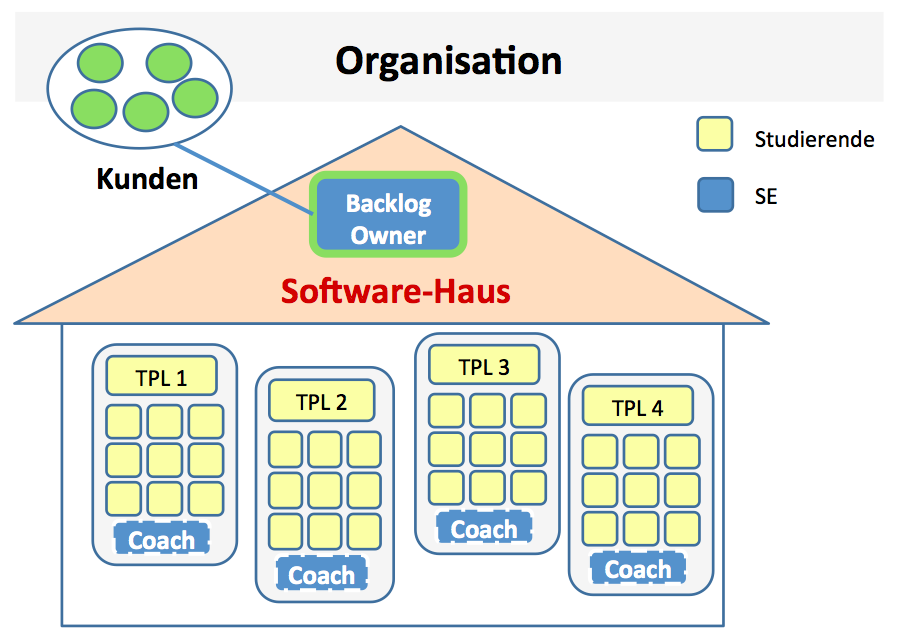
\includegraphics[scale=0.20]{Organisation}
	\caption*{\scriptsize{Quelle: SE-Webseite (Stand 21. Oktober 2014)}}
	\end{figure}
	
\end{frame}
	
\begin{frame}
	\frametitle{Software Projekt}
	\framesubtitle{Die Problemstellung}
	\begin{itemize}
	\pause 
		\item 60 Inf., 24 Math., 24 Tech. Inf.
		\pause 
		\item Gleichm\"a{\ss}ige Verteilung der Studieng\"ange in jedem Team.
		\pause 
		\item M\"oglichst gro{\ss}e Anzahl von Teams.
		\end{itemize}
\end{frame}

\begin{frame}
	\frametitle{Software Projekt}
%	\framesubtitle{Der 1. Schritt zur L\"osung}
	Sei $n \in \mathbb{N}$ die Anzahl der Teams.
	\pause 
	\begin{align*}
	\Rightarrow n|60 \text{, } n|24 \text{ und } n|24 \tag{i}\\
	\end{align*}
	\pause 
	Wir suchen nach der gr\"o{\ss}ten Zahl $n$, die $(i)$ erf\"ullt.
	\pause 
	\begin{align*}
	\Rightarrow n = \textit{ggT}(60,24,24) = 12 \text{ Teams}\\
	\end{align*}
	
\end{frame}

\begin{frame}
	\frametitle{Software Projekt}
	\framesubtitle{L\"osungsanalyse}
	Es gibt 12 Teams mit jeweils  --\\
	\begin{itemize}
	\item 9 Studenten
	\pause 
	\item 5 Informatik Studenten
	\pause 
	\item 2 Mathematik Studenten
	\pause 
	\item 2 Technische-Informatik Studenten
	\end{itemize}
\end{frame}

\begin{frame}
\frametitle{Analog: Computerspiele}
\framesubtitle{Missionsdauer}
\vspace*{10pt}
\pause 
20 Stunden/50 Stunden pro Woche.\\
\pause 
 \begin{figure}
	\centering
	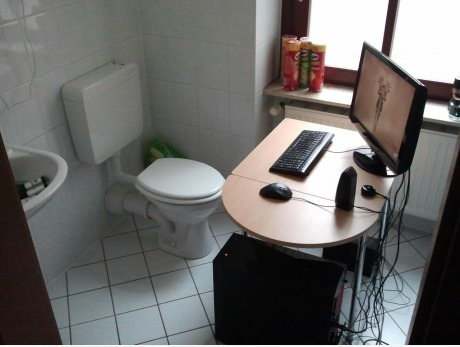
\includegraphics[scale=0.6]{gamers}
	\caption*{\scriptsize{Quelle: blog.wirebot.com}}
	\end{figure}
\end{frame}

\begin{frame}
	\frametitle{Problem 2: Mit dem Teufel umgehen}
    \framesubtitle{M\"oglichst wenig Kontakt}
    \pause 
    \vspace*{10pt}
     \begin{figure}
	\centering
	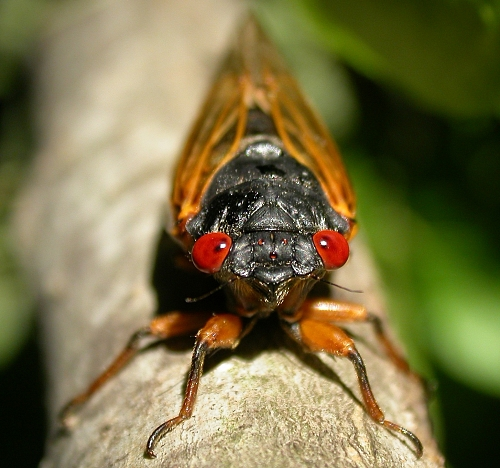
\includegraphics[scale=0.17]{cicada}
	\caption*{\scriptsize{Quelle: Office Space}}
	\end{figure}
    \begin{itemize}
    \pause 
    \item Chef macht alle 4 Stunden Pause.
    \pause 
    \item Das eigene B\"uro alle 3 Stunden verlassen.
    \end{itemize}
\end{frame}

\begin{frame}
	\frametitle{Teilerfremdheit von Zahlen}
	\pause 
\begin{itemize}
\item Teilerfremdheit durch Vergleich der Primfaktoren ($NP$).
\pause
\item Schnell Zahlen auf Teilerfremdheit pr\"ufen, ohne zu faktorisieren.
\end{itemize}
\pause 
$$ggT(a,b) = \prod_{i \in \mathbb{N}} p_{i}^{min(a_i,b_i)}$$ wobei $p_{i} \in \mathbb{P}$.
%Die Bestimmung der Primfaktorzerlegung einer Zahl liegt aber in NP.
\end{frame}

\begin{frame}
\frametitle{Von der Problemstellung abstrahieren}
\pause 
\begin{quote}
		Wie kann man schnell den \textit{g.g.T.} bestimmen?
	\end{quote}
	\pause 
	\begin{itemize}
	\item Euklidischer Algorithmus
	\item Binary GCD Algorithm von Stein
	\item GCD Algorithm von Lehmer
	\end{itemize}
\end{frame}

\section{Einf\"uhrung}

\begin{frame}       
	\frametitle{Euklidischer Algorithmus}
    \framesubtitle{Historische Entwicklung}
    \begin{itemize}
    \pause 
    \item  ca. 300 \textit{v.Chr.} in \textit{Buch VII -- Die Elemente} vorgestellt.
    \pause 
    \item Wahrscheinlich nicht selbst erfunden.
    \pause 
    \item Als geometrischen Algorithmus vorgestellt. St\"abe zerlegt.
    \end{itemize}
\end{frame}

\section{Vorstellung der Algorithmen}
\begin{frame}
	\frametitle{Vorstellung der Algorithmen}
	\begin{itemize}
	\item \textsc{LangsamEuklid}
	\item \textsc{Euklid}
	\end{itemize}
\end{frame}

%Code
%Flow Chart
%Beispiel
%Korrektheit
%Finiteness

\subsection{\textsc{LangsamEuklid}}
\begin{frame}
	\frametitle{\textsc{LangsamEuklid}}
	\underline{\textsc{LangsamEuklid}}: Gegeben $a,b\in\mathbb{N}$
	\pause
	\begin{algorithmic}[1]
\While {$a\neq b$}
	\pause
	\State Falls $a$ gr\"o{\ss}er ist als $b$, $a\gets a-b$
	\State Falls $b$ gr\"o{\ss}er ist als $a$, $b\gets b-a$
	\pause
\EndWhile
	\pause
	\State Gib den gemeinsamen Wert der Zahlen aus
\end{algorithmic}
\end{frame}

\begin{frame}
	\frametitle{\textsc{LangsamEuklid}}
	\begin{figure}
	\centering
	\begin{tikzpicture}

	\draw [thick, ->] (0.3, 2) -- (0.3, 1);
	\draw (0,1) -- (0,0) -- (2,0) -- (2,1) -- (0,1);
	\node at (1, 0.5) {\scriptsize{$a=b?$}};
	
	\draw [->] (2,0.5) -- (4,0.5);
	\node [above] at (3, 0.5) {\scriptsize{Nein}};
	
	\draw (4,1) -- (4,0) -- (6,0) -- (6,1) -- (4,1);
	\node at (5, 0.5) {\scriptsize{Subtraktion}};
	
	\draw (6, 0.5) -- (7, 0.5) -- (7, 2) -- (1, 2);	
	\draw [->] (1,2) -- (1,1);
	
	\node [above] at (-0.75,0.5) {\scriptsize{Ja}};
	\draw (0,0.5) -- (-1.5,0.5);
	\draw [->] (-1.5,0.5) -- (-1.5, -1);

	\draw (-3,-1) -- (-3, -2) -- (-1, -2) -- (-1, -1) -- (-3,-1);
	\draw (-2.9,-1.1) -- (-2.9, -1.9) -- (-1.1, -1.9) -- (-1.1, -1.1) -- (-2.9,-1.1);
	\node at (-2, -1.5) {\scriptsize{return $a$}};
	\end{tikzpicture}
	\caption{Flussdiagramm \textsc{LangsamEuklid}}
	\end{figure}
\end{frame}
\begin{frame}
	\frametitle{\textsc{LangsamEuklid}}
	\framesubtitle{Beispiel}
	Beispiel: $a=24, b=9$:\\
	\vspace{5pt}
	\begin{tabular}{|c|c|c|} \hline 
	Iteration Nr.& a & b \\ \hline 
	& 24 & 9  \\ 
	1\pause & 15 & 9 \\ 
	2\pause & 6 & 9  \\ 
	3\pause & 6 & 3  \\ 
	4\pause & \textbf{3} & \textbf{3} \\ \hline
	\end{tabular}\\ \vspace{5pt}
	$\Rightarrow$ der \textit{g.g.T.} von 24 und 9 ist 3.
\end{frame}

\begin{frame}
	\frametitle{\textsc{LangsamEuklid}}
	\framesubtitle{Endlichkeit}
	\begin{itemize}
	\pause 
	\item Zahlen bleiben positiv beim Subtraktionsschritt.
	\pause 
	\item Eine Variable wird immer um mindestens 1 
verringert.
\pause 
	\item D.h. der Algorithmus terminiert nach maximal $a+b$ Durchl\"aufen.
	\end{itemize}
\end{frame}

\begin{frame}
	\frametitle{\textsc{LangsamEuklid}}
	\framesubtitle{Korrektheit}
	\begin{itemize}
	\pause 
	\item \textit{g.g.T.}$(a,b)$ = \textit{g.g.T.}$(a-b,b)$
	\item \textit{g.g.T.}$(a,a)$ = $a$
	\end{itemize}
\qed
\end{frame}
\begin{frame}
	\frametitle{\textsc{LangsamEuklid}}
	\framesubtitle{Verbesserungsvorschl\"age}
	\pause
	\begin{itemize}
	\item $(1069,2) \rightarrow (1067,2) \rightarrow \dots (3,2) \rightarrow (1,2) \rightarrow (1,1)$
	\pause
	\item In den meisten Iterationen braucht man nicht $a>b$ \"uberpr\"ufen.
	\end{itemize}
\end{frame}

\subsection{\textsc{Euklid}}
\begin{frame}
	\frametitle{\textsc{Euklid}}

\underline{\textsc{Euklid}}: Gegeben $a,b\in\mathbb{N}$
\pause 
	\begin{algorithmic}[1]
		\While {$b>0$}
		\pause 
		\State berechne $q,r$ mit $a=q\cdot b+r$, wobei $0\leq r < b$
		\pause 
		\State $a\gets b, b\gets r$
		\pause 
		\EndWhile
		\State \textbf{return} $a$
	\end{algorithmic}	
	
\end{frame}
\begin{frame}
	\frametitle{\textsc{Euklid}}

	\begin{figure}
	\centering
	\begin{tikzpicture}

	\draw [thick, ->] (0.3, 2) -- (0.3, 1);
	\draw (0,1) -- (0,0) -- (2,0) -- (2,1) -- (0,1);
	\node at (1, 0.5) {\scriptsize{$b>0?$}};
	
	\draw [->] (2,0.5) -- (4,0.5);
	\node [above] at (3, 0.5) {\scriptsize{Ja}};
	
	\draw (4,1) -- (4,0) -- (6,0) -- (6,1) -- (4,1);
	\node at (5, 0.75) {\scriptsize{Division}};
	\node at (5, 0.25) {\scriptsize{Reduktion}};
	
	\draw (6, 0.5) -- (7, 0.5) -- (7, 2) -- (1, 2);	
	\draw [->] (1,2) -- (1,1);
	
	\node [above] at (-0.75,0.5) {\scriptsize{Nein}};
	\draw (0,0.5) -- (-1.5,0.5);
	\draw [->] (-1.5,0.5) -- (-1.5, -1);

	\draw (-3,-1) -- (-3, -2) -- (-1, -2) -- (-1, -1) -- (-3,-1);
	\draw (-2.9,-1.1) -- (-2.9, -1.9) -- (-1.1, -1.9) -- (-1.1, -1.1) -- (-2.9,-1.1);
	\node at (-2, -1.5) {\scriptsize{return $a$}};
	\end{tikzpicture}
\caption{Flussdiagramm \textsc{Euklid}}
\end{figure}
\end{frame}

\begin{frame}
\frametitle{\textsc{Euklid}}
\framesubtitle{Beispiel}
\pause
\begin{tabular}{|c|c|c|} \hline
	Iteration Nr.& a & b \\ \hline
	& 1069 & 2  \\
	1\pause & 2 & 1 \\
	2\pause & 1 & \textbf{0} \\ \hline
	\end{tabular}\\ \vspace{5pt}
	$\Rightarrow$ der \textit{g.g.T.} von 1069 und 2 ist 1.

\end{frame}

\section{Laufzeitanalyse}

\begin{frame}
	\frametitle{Laufzeitanalyse}
	\framesubtitle{\textsc{Euklid vs. LangsamEuklid}}
	Sei ohne Einschr\"ankung $a>b$.\pause \\ Im ersten Durchlauf gilt --
	
	\begin{equation}a = q \cdot b + r \text{, mit } r < b
	\end{equation}
	\pause 
	 Au{\ss}erdem gilt -- \\ \begin{equation}a \geq b + r \end{equation} \\
	 \pause 
	 Aus $(1), (2)$ folgt $$r < \frac{a}{2}$$ \\
\end{frame}	
\begin{frame}
	\frametitle{Laufzeitanalyse}
	\framesubtitle{\textsc{Euklid vs. LangsamEuklid}}
	\begin{itemize}
	\item $a_{2}, b_{2} < \cfrac{a}{2}$ \vspace*{10pt}
	\pause 
	\item Nach $2 \cdot k$ Iterationen sind die Variablen h\"ochstens so gro{\ss} wie $\cfrac{a}{2^k}$ \vspace{15pt} .	
	\pause 
	\item $k \leq \log_{2}a$
	\pause 
	\item $2\cdot \log_{2}a$ besser als $a+b$
	\end{itemize}
\end{frame}

	\begin{frame}
	\frametitle{Worst-Case}
	\framesubtitle{\textsc{Euklid}}
\pause
	Betrachte die Fibonacci-Zahlen --
	\begin{align*}
 f_{n+1} &= 1 \cdot f_{n} + f_{n-1} \\
 f_{n} &= 1 \cdot f_{n-1} + f_{n-2} \\
 &\vdots \\
 f_{2} &= 1 \cdot f_{1} + 0 \\
 f_{1} &= 1
\end{align*}
\end{frame}	
\begin{frame}
\frametitle{Definition}
\pause
\begin{itemize}
	\item Sei $T(a,b)$ die Anzahl der Durchl\"aufe von \textsc{Euklid}$(a,b)$.
	\pause
	\item z.B. $T(1069,2) = 3$
\end{itemize}

\end{frame}
\begin{frame}
	\frametitle{Durchschnittslaufzeit}
	\framesubtitle{\textsc{Euklid}}
	\pause
	Wenn $b$ feststeht und $a$ \"uber alle nat\"urlichen Zahlen variiert, wieviele Durchl\"aufe gibt es im Schnitt?\vspace{10pt}
	\pause
	\begin{quote}
	Sei $T_{b}$ diese durchschnittliche Anzahl.
	\end{quote}
	\end{frame}
\begin{frame}
\frametitle{$T_b$ berechnen}
 \begin{center}
 \begin{tabular}{|c|c|} \hline
 $T(3,5) = 4$ & $T(718,5) = 4$  \\ \hline
 	& \\
	$3=0\cdot 5 + 3$ & $718=143\cdot 5 + 3$ \\
	& \\
	$5=1\cdot 3 + 2$ & $5=1\cdot 3 + 2$ \\
	$3=1\cdot 2 + 1$ & $3=1\cdot 2 + 1$ \\
	$2=1\cdot 1 + 0$ & $2=1\cdot 1 + 0$ \\ \hline
	 \end{tabular}
	  \end{center}
	  \pause
	   Nach der ersten Iteration ist immer nur der Divisionsrest relevant.
\end{frame}
\begin{frame}
\frametitle{$T_b$ berechnen}
	$$\Rightarrow T_{b} = \frac{1}{b} \sum_{0 < k\leq b} T(k,b)$$
	\end{frame}

\begin{frame}	
		\frametitle{Durchschnittslaufzeit}
	\framesubtitle{\textsc{Euklid} : Beispiel $T_5$}
	\pause
$$T_5 = \frac{1}{5}\cdot (T(1,5) + T(2,5) \dots +T(5,5))$$	
\pause
	\begin{itemize}
	\item $T(1,5) = 2$
	\setcounter{equation}{0}
	\begin{align}
	1&=0\cdot 5 + 1	\\
	5&=5\cdot 1 + 0
	\end{align}
	\pause
	\setcounter{equation}{0}
	\item $T(2,5) = 3$
	\begin{align}
	2&=0\cdot 5 + 2	\\
	5&=2\cdot 2 + 1 \\
	2&= 2\cdot 1+0
	\end{align}
	\end{itemize}
	
	\end{frame}
	

\begin{frame}	
		\frametitle{Durchschnittslaufzeit}
	\framesubtitle{\textsc{Euklid} : Beispiel $T_5$}
	Analog-
	\begin{itemize}
	\item $T(3,5) = T(8,5) = \dots = 4$*
	\item $T(4,5) = T(9,5) = \dots = 3$
	\item $T(5,5) = T(10,5) = \dots = 1$
	\pause
	\end{itemize}
	\vspace{20pt}
	 $$\Rightarrow T_5 = \frac{2+3+4+3+1}{5} = 2.6\text{ Iterationen}$$
	\end{frame}	

	\begin{frame}	
		\frametitle{Durchschnittslaufzeit}
	\framesubtitle{\textsc{Euklid} : Absch\"atzung von $T_b$}
	\pause
	F\"ur gro{\ss}e $b \in \mathbb{N}$ gilt
	\begin{itemize}
	\item Nach der ersten Iteration von $\textsc{Euklid}(k,b)$ bleiben noch ungef\"ahr $T_{k}$ Iterationen.
	\pause
	\begin{align*}
	k&=0\cdot b + k\\
	b&=q_{2}\cdot k + r_2\\
	&\vdots
\end{align*}		
\pause
	\item $T_b \approx 1 + \frac{1}{b} (T_1 + T_2 \dots + T_{b})$
	\end{itemize}
\end{frame}		

\begin{frame}
\frametitle{Durchschnittslaufzeit}
\framesubtitle{\textsc{Euklid} : Absch\"atzung von $T_b$}
$$ \Rightarrow T_b \approx H_b = \ln b + O(1)$$
\pause
 \begin{center}
 \begin{tabular}{|c|c|} \hline
 $T_{100} \approx 4.56$ & $H_{100} \approx 5.18$ \\ 
 $T_{1000} \approx 6.42$ & $H_{1000} \approx 7.49$ \\
 $T_{10^6} \approx 12.2$ & $H_{10^6} \approx 14.4$ \\ 
  $T_{10^8} \approx 16.07$ & $H_{10^8} \approx 18.99$ \\ 
    $T_{10^9} \approx 18.01$ & $H_{10^9} \approx 21.3$ \\ \hline
  
	 \end{tabular}
	  \end{center}

\end{frame}

\begin{frame}
	\begin{figure}
	\centering
	\includegraphics[scale=0.42]{graph}
	\caption*{\scriptsize{X: ln(b), Y: Anzahl Durchl\"aufe}}
	\end{figure}
\end{frame}

\begin{frame}
\frametitle{Weiterf\"uhrende Literatur}
\begin{itemize}
\item \textit{The Art of Computer Programming: Band 1} Kap. 1.1
\item \textit{The Art of Computer Programming: Band 2} Kap. 4.5.2
\end{itemize}
\end{frame}

\begin{frame}
\frametitle{Zusammenfassung}
\begin{itemize}
\item Euklidischer Algorithmus berechnet den \textit{g.g.T} zweier Zahlen.
\item Teilerfremdheit mit Primfaktorzerlegung ineffizient.
\item Laufzeit von \textsc{LangsamEuklid} abh\"angig von Zahlen.
\item Laufzeit von \textsc{Euklid} abh\"angig von der Anzahl der Ziffern der Zahlen.
\item Nach der 1. Iteration ist nur der Divisionsrest relevant.
\item Fibonacci-Zahlen bilden das Worst-Case Szenario.
\end{itemize}
\end{frame}

\begin{frame}
\frametitle{Anhang}
	Beweis:\\
	$ T_b \approx S_b \text{, wobei }$ $$S_0 := 0, S_n := 1 + \frac{1}{n} (S_0 + S_1 \dots + S_{n-1})$$
	\begin{align*}
	\Rightarrow S_{n+1} &= 1 + \frac{1}{n+1}(S_0 + S_1 \dots + S_{n-1}+ S_n)\\
	\end{align*}
	
\end{frame}

\begin{frame}
\frametitle{Anhang}
\begin{align*}
&= 1 + \frac{1}{n+1}(n\cdot (S_n - 1) + S_n)\\
	&\Rightarrow S_{n+1}= S_n + \frac{1}{n+1}
\end{align*}
$$\Rightarrow S_n = H_n = 1 + \frac{1}{2} + \dots +\frac{1}{n}$$ $$ \Rightarrow T_b \approx \ln b + O(1)$$

\end{frame}

\end{document}

